\chapter{系统分析与规划}
\label{chap:1}

此节目标是为了建立一个面向网路教学的听课状态视频分析系统,该章节讨论该系统的目标架构,并说明实际完成的部分。此章节也会针对初期可运用的技术逐一进行说明。

\section{系统规划}

由于本作业将面向网路教学的听课状态视频分析系统,在作为实际的产品进行规划,实际需要的功能分为九个项目,其项目为会员功能、视频观看、作业缴交、教学直播、学习检测、代码提交、签到功能、课堂抢答、考试功能。

\subsection{功能概念规划}

\begin{figure}[htb]
\centering 
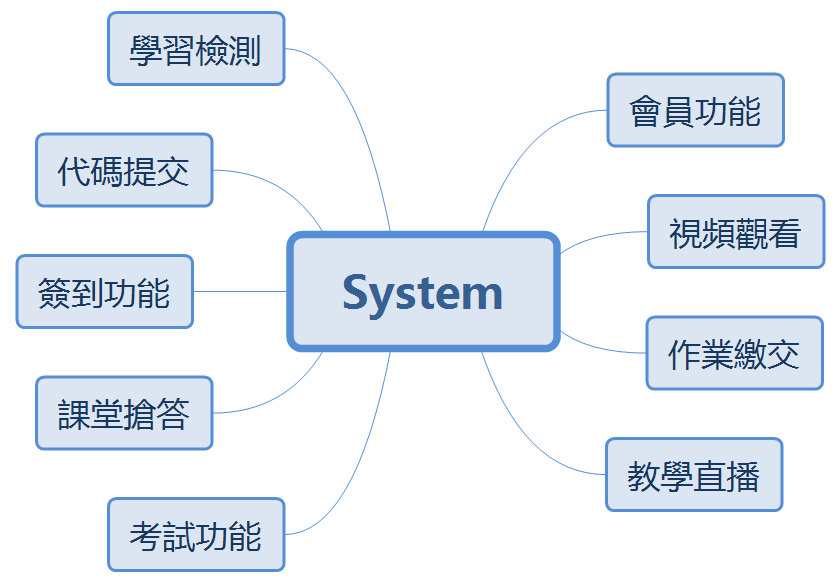
\includegraphics[width=0.60\textwidth]{img/ch1m1.png} 
\caption{系统功能面规划}
\label{Test}
\end{figure}

\begin{itemize}
\item [-] 会员功能 : 其会员系统分为老师使用者、学生使用者、系统管理者。
\item [-] 视频观看 : 为播放上课视频录影或者是老师预先上传的教学录影视频。
\item [-] 作业缴交 : 为作业缴交功能。
\item [-] 教学直播 : 为针对教学现场的直播,该功能与考试功能、课堂抢答、学习检测相关。
\item [-] 学习检测 : 为协助老师判断学生精神状况的功能。老师在教学直播或者视频观看两大功能中,可设定对学生当下的学习状况进行判断的请求,当学生同意后,系统则会搜集学生执行系统的电脑镜头,并对镜头前的状况进行疲劳或者注意力的判断。最后产生统计报表。
\item [-] 代码提交 : 为类似 GitHub 的版本控制,学生提交代码作业后,该系统除了收纳外,过程中会进行代码比对,可判断有无相互抄袭代码。
\item [-] 签到功能 : 与教学直播相关的连动功能。
\item [-] 课堂抢答 : 与教学直播相关的连动功能。
\item [-] 考试功能 : 分为大考与临时考试两种,由老师进行设定。
\end{itemize}

\subsection{功能概念关联}

该节说明各功能之间的关联,其使用者登入会员系统后,会根据使用者不同的权限而有不同的服务。当中课堂抢答、签到功能、学习检测都是要在使用者进入由老师方或者系统管理方使用者所发起的教学直播,才会接触到。当中学习检测功能则是不论视频观看或者教学直播功能中都能够发起。

\begin{figure}[htb]
\centering 
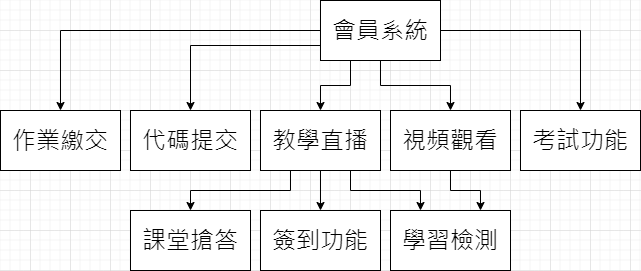
\includegraphics[width=0.80\textwidth]{img/ch1m2.png} 
\caption{关联说明}
\label{Test}
\end{figure}

\subsection{系统架构说明}

本系统架构分别为三大部分,一个是资料库,前端框架则是为 Vue,后端框架则是运用 Python Flask 作为主体的服务提供,而 Go 则是预计处理负责版本控制功能的部分。同时因为需要深度学习在计算机视觉的功能,在此会考量运用 Python 中的 Pytorch 或者是 Python 的 TensorFlow,这也是本作业考量使用 Python 作为主体开发方案的原因。

\begin{figure}[htb]
\centering 
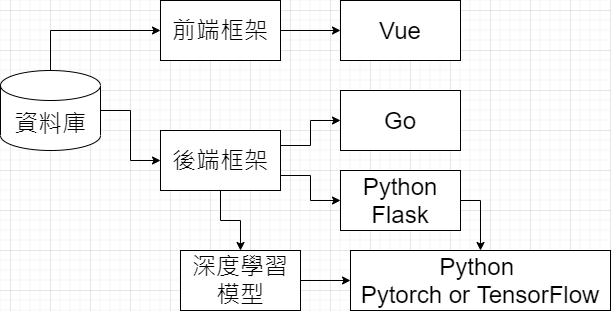
\includegraphics[width=0.80\textwidth]{img/ch1m3.png} 
\caption{关联说明}
\label{Test}
\end{figure}

\section{系统介面規劃}

此节为说明在系统规划中各个功能的预计线框图(Wireframe)的概念设计,其项目为会员功能、视频观看、作业缴交、教学直播、学习检测、代码提交、签到功能、课堂抢答、考试功能。

\subsection{会员功能}

在此会员功能分成三大部分,当中权限分为管理者、老师、学生三种权限,管理者拥有管理老师跟学生帐号的管理权限,同时也能够如老师帐号一样进行课堂直播与建立视频的课程,而老师帐号则是可以管理学生进入课堂,并且发起教学与进行课堂直播与建立视频的课程,同时可以询问学生进行学习效果的判断。

\begin{figure}[htb]
\centering 
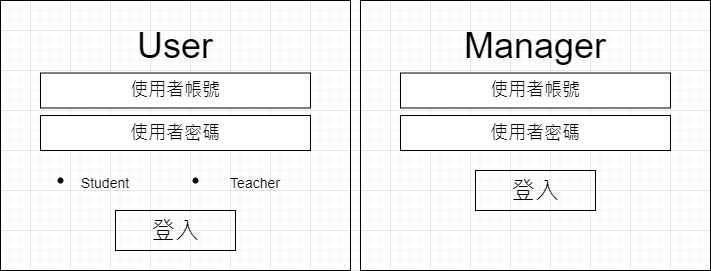
\includegraphics[width=0.80\textwidth]{img/ch1m4.png} 
\caption{会员功能线框图}
\label{Test}
\end{figure}

\subsection{视频观看}

所谓的是频观看则分为两方描述,从学生角度来看,可以从老师上传的视频进入后进行观看,同时有一个笔记的按钮,该按钮的介面设计是可以开启一个支援 LaTeX 的编辑器,同时有着撷取老师录影画面,进行简易绘图笔记的功能,而笔记功能则是每个权限都可以使用。

另外还有一个课堂影片条列的功能,但由于老师跟管理员权限与学生不一致的缘故,故只有学生的画面中并没有增设学习状况判断的按钮。而从老师与管理员权限的角度来看,若在影片列表中设定增设学习状况的判断,那从学生的页面中则会看到,系统会跳出是否要让老师能够产生学习状况判断的讯息,若学生勾选否,则系统会在整班的报告中,回报该学生没有选同意此选项,而若学生选择同意,则系统会在整堂课随机时间利用使用者的摄像头,随机固定间隔时间拍照进行分析,行分析,产生出使用者目前学习的精神状况与判断,并将数据纪录下来进行统计并产生报表。

\begin{figure}[htb]
\centering 
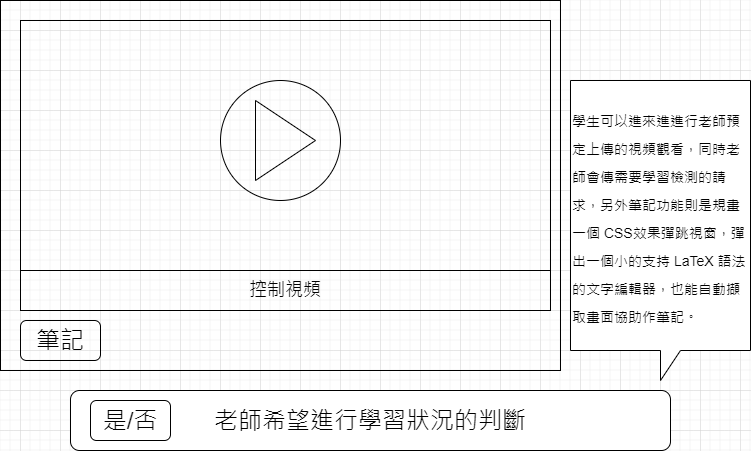
\includegraphics[width=0.80\textwidth]{img/ch1m5.png} 
\caption{视频观看页面的概念线框图}
\label{Test}
\end{figure}

\begin{figure}[htb]
\centering 
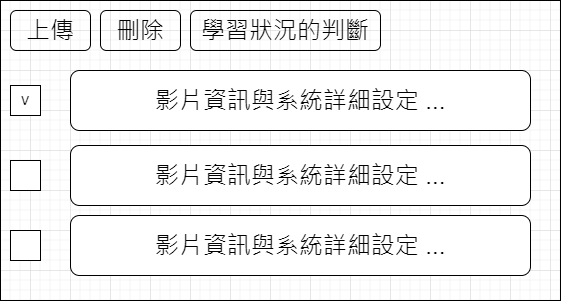
\includegraphics[width=0.50\textwidth]{img/ch1m6.png} 
\caption{视频观看的列表概念线框图}
\label{Test}
\end{figure}

\subsection{代码提交}

此节功能的现有方案为 gogs ,一个由开源社群开发的类似 GitHub 的项目代码管理平台,该方案由 Go 语言实现,若出于实际需求可能需要写整合的代码。但在此还是将其需求进行分析。从列表分析的页面为从管理员权限与老师的权限可用,此权限可以用代码交叉对比的功能,来判断学生间的代码是否互相抄袭,其功能实现则根据现有的开源套件进行整合,同时管理方与老师方也可以加入搜集来的范例去进行比对,如此一来类似助教可以在网路上爬取相关代码。一旦判断相似度高,则系统会给学生建议,请学生对其作业加入引用或者注明来源,鼓励学生除了自学之外,从其他资源的代码中学习到编程能力经验好的代码。另外代码提交页面,其功能类似于 GitHub 等开源项目管理平台的页面,当中可以提交程式码,并对其项目进行管理与版本控制,方便教授跟助教对学生的程式码进行批改。同时此部分支持学生团队开发协作,从而学习到对团队协作的软件开发工程经验。

\begin{figure}[htb]
\centering 
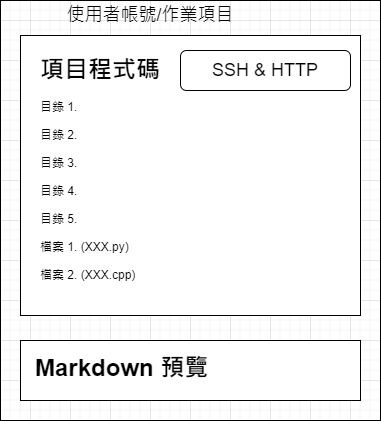
\includegraphics[width=0.40\textwidth]{img/ch1m8.png} 
\caption{代码提交的页面概念线框图}
\label{Test}
\end{figure}
\begin{figure}[htb]
\centering 
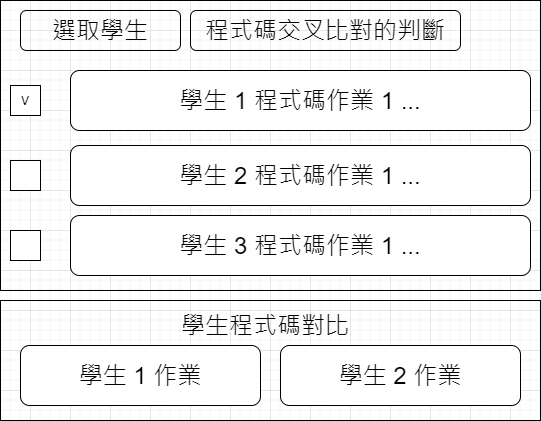
\includegraphics[width=0.50\textwidth]{img/ch1m7.png} 
\caption{代码提交列表的概念线框图}
\label{Test}
\end{figure}

\subsection{作业缴交}

在此现有整合的开源方案其中为 HackMD,同时该方案也有服务,为重要的笔记 Markdown 软体,但需求包含了 PDF、 Word、 Markdown、LaTeX 等档案类型,其复杂程度高,故尽可能使用现有的开源项目进行整合。而作业缴交页面的概念源自于学生权限的页面,由老师或者管理员权限建立课程发起作业后,学生提交相关档案,同时学生能够检视自己上传上来的文件。并且上传上来的文件可以进行档案版本的分类,从而协助管理档案的版本。

另外从列表的部分来看,该页概念为老师与管理权限可以运用文件内容交叉对比进行查核,若有相似性,则系统提供提醒,鼓励学生权限的使用者,引用与注明作业跟文献内容的来源。

\begin{figure}[htb]
\centering 
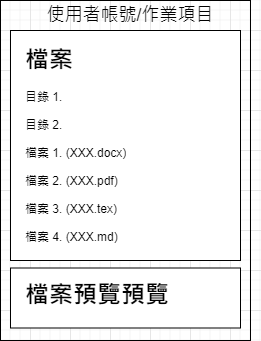
\includegraphics[width=0.50\textwidth]{img/ch1m9.png} 
\caption{作业缴交的页面概念线框图}
\label{Test}
\end{figure}

\begin{figure}[htb]
\centering 
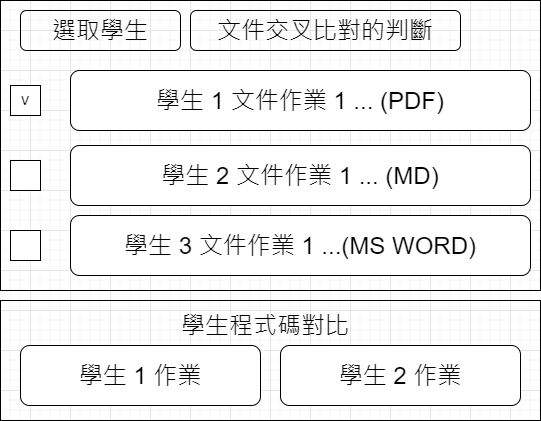
\includegraphics[width=0.80\textwidth]{img/ch1m10.png} 
\caption{作业缴交列表的概念线框图}
\label{Test}
\end{figure}


\subsection{教学直播}

此部分功能从老师与管理方来看,老师可以发起点名、抢答与学习状况的判断,而学生部分的则是可以回应,并且当中对过程的次数会进行纪录,同时发起抢答时,老师与管理方能设定秒数,此秒数会显示在学生方的按钮上,该秒数会倒数的状态,另外发起点名这个则是会累积,若学生方较晚才回应,老师的后台可以看到学生方在哪几次的点名于何时回应,而回应当下的时间则会于发起的点名时间互减,用来告知老师与管理方,学生点名的时间差。

另外与视频观看相同的地方在于,老师与管理端在此也能进行学习检测的功能发起,发起的当下,系统会提醒学生,并等待学生回应,若学生同意则运用该电脑的摄影机去随机抓出特定帧进行模型的判断,同时学生会在画面的另看到一角看到自己被判断的画面,最后该数据会统计,并回传给老师进行检视。

\begin{figure}[htb]
\centering 

\includegraphics[width=0.80\textwidth]{img/ch1m11.png} 
\caption{学生教学直播的页面概念线框图}
\label{Test}
\end{figure}

\begin{figure}[htb]
\centering 

\includegraphics[width=0.80\textwidth]{img/ch1m12.png} 
\caption{老师教学直播的页面概念线框图}
\label{Test}
\end{figure}


\subsection{学习检测}

学习检测功能是此次作业的重点,此部分有可能要拆成两部分来做,但在技术上很可能要用三个部分来看,第一个为前端画面 Vue、第二个为后段的 Flask、第三部分为 PyTorch 或者 TensorFlow 的深度学习模型整合,而从技术领域上,开发过程很可能要面对视频的处理,另外还有视频辨识所产生出来的分析,同时最后要生成老师方或者管理方可以分析的学习状态报表。同时判断学生是否在稳定的状态中进行学习也是很重要的一部分,此部分判断与规划的分析留待后面章节继续说明。

由下图可以知道,上图为可以判断的流程影像处理,当中原影像是随机从每一帧选取,其一是判断画面有没有人,其二判断有无可辨识的人脸,其三判断人眼的眼睛是否疲劳,其四则是判断人的表情是否疲惫。

\begin{figure}[htb]
\centering 

\includegraphics[width=0.80\textwidth]{img/ch1m13.png} 
\caption{学习检测页面概念线框图}
\label{Test}
\end{figure}

\subsection{考试功能}

考试功能为老师与管理方权限可以进行发起考试,当中考试可设为随堂考或者期末考,考题可以根据 CSV 、JSON、MS EXCEL 等不同格式来输入成为选择题,又或者是进入设定显示老师的问答题目。

\begin{figure}[htb]
\centering 
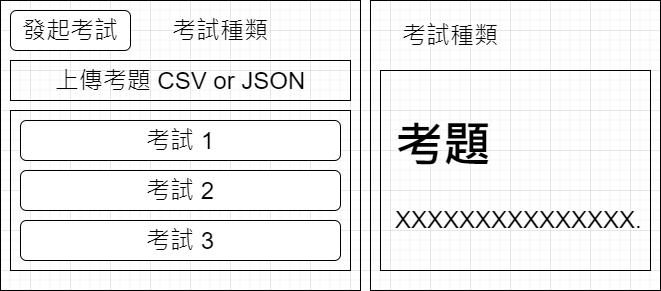
\includegraphics[width=0.80\textwidth]{img/ch1m14.png} 
\caption{考试功能页面概念线框图}
\label{Test}
\end{figure}

%\section{系统分析}
%\section{系统概念}
%\subsubsection{SSS1}

%\begin{itemize}
%\item [-][7,7] 空间卷积到 1*1*2048 然后一维卷积到 1*1*128
%\item [-]池化层到 1*1*2048 然后一维卷积到 1*1*128
%\end{itemize}


%\begin{itemize}
%\item Calculus
%\item Linear Algebra
%\item Basic Computer Concepts
%\end{itemize}

%\begin{description}
% \item[First] \hfill \\
% The first item
% \item[Second] \hfill \\
% The second item
% \item[Third] \hfill \\
% The third etc \ldots
%\end{description}
